\documentclass[addpoints]{exam}

\usepackage{caption}
\usepackage{graphbox}
\usepackage{hyperref}
\usepackage{multirow}
\usepackage{pythonhighlight}
\usepackage{ragged2e}
\usepackage{subcaption}
\usepackage{tabularx}
\usepackage{titling}
\usepackage{xcolor}
\usepackage{float}

\usepackage{listings}
\usepackage{titling}
\usepackage{xcolor}
\usepackage{color}
\definecolor{backcolour}{rgb}{0.95,0.95,0.92}
\definecolor{codegreen}{rgb}{0,0.6,0}
\definecolor{deepblue}{rgb}{0,0,0.5}
\definecolor{deepred}{rgb}{0.6,0,0}
\definecolor{deepgreen}{rgb}{0,0.5,0}

% Python style for highlighting
\newcommand\pythonstyle{\lstset{
language=Python,
basicstyle=\ttm,
backgroundcolor = \color{backcolour},
commentstyle = \color{codegreen},
morekeywords={self},              % Add keywords here
keywordstyle=\ttb\color{deepblue},
emph={MyClass,_init_},          % Custom highlighting
emphstyle=\ttb\color{deepred},    % Custom highlighting style
stringstyle=\color{deepgreen},
frame=tb,                         % Any extra options here
showstringspaces=false,
tabsize = 4
}}

% Python for inline
\newcommand\pythoninline[1]{{\pythonstyle\lstinline!#1!}}

% Header and footer.
\pagestyle{headandfoot}
\runningheadrule
\runningfootrule
\runningheader{CS 201, Spring 2023}{HW 2: Skiplists and Dynamic List ADT}{\theauthor}
\runningfooter{}{Page \thepage\ of \numpages}{}
\firstpageheader{}{}{}

\qformat{{\large\bf \thequestion. \thequestiontitle}\hfill[\totalpoints\ points]}
% \qformat{{\large\bf \thequestion. \thequestiontitle}\hfill}
\boxedpoints

\printanswers

\graphicspath{{images/}}

\newcommand\colheader[1]{\multicolumn{1}{c}{#1}} % Note: no vertical bars

\title{Homework 2: Skiplists and Dynamic List ADT}
\author{L5 - Group 3}  % <=== Enter your team name.
\date{Habib University\\Spring 2023}

\begin{document}
\maketitle
\part{Dynamic List ADT}

In this assignment, you will implement a dynamic list ADT in Python that allows for inserting and deleting elements at a specified index and retrieving elements at a specified index.
The list should be implemented as both a dynamic array and a linked list.


\section{Implementation Details and Tasks}

\begin{itemize}
  \item Implement the \pyth{DynamicArrayList} and \pyth{LinkedList} classes in the accompanying file, \texttt{listadt.py}, in the accompanying \texttt{src/} sub-folder.
  \item In the \pyth{DynamicArrayList} and \pyth{LinkedList} classes, implement the following methods:
        \begin{itemize}
          \item \pyth{insert(index, value)}: inserts value at the specified index
          \item \pyth{delete(index)}: deletes the element at the specified index
          \item \pyth{get(index)}: returns the element at the specified index
          \item \pyth{size()}: returns the number of elements in the list
          \item \pyth{display()}: returns the string representation of the list
        \end{itemize}
  \item The dynamic array should be implemented using Python \pyth{arrays}. Upon creation, the dynamic array will have a size of one, and all empty items will be initialised as -1.
  \item The dynamic array should dynamically resize itself when necessary to ensure efficient use of memory i.e., \textbf{the array should double it's size when it is full
          and reduce by half once it is quarter the size of array.}
  \item The cost of resizing the array should be linear in the size of the array.
  \item The linked list should be implemented as a singly linked list.
  \item The program should take as an input a file that specifies which data structure should be used to implement the dynamic list ADT and which operations should be performed on the list.
  \item The program should read the input file, create the appropriate data structure, and perform the specified operations. The program should then output the result of each operation.
  \item The function \pyth{load} which parses the input file and saves the output of the program to a given file, has already been implented in the accompanying file, \texttt{listadt.py}, in the accompanying \texttt{src/} sub-folder.
\end{itemize}


\subsection{Input and Output}

The input file will specify which data structure should be used to implement the Dynamic List ADT and which operations should be performed on the list. The input file will have the following format:
\begin{center}
  \begin{tabular}{c}
    \begin{lstlisting}[language={}]
    <data structure>
    <operation> <arg1> <arg2>
    \end{lstlisting}
  \end{tabular}
\end{center}
\begin{itemize}
  \item $\langle$\textbf{data structure}$\rangle$ is either array or linkedlist, indicating which data structure should be used to implement the Dynamic List ADT
  \item $\langle$ \textbf{operation}$\rangle$ is one of the following:
        \begin{itemize}
          \item \textbf{insert}: Insert an item into the list. The $\langle$arg1$\rangle$ is the index at which to insert the item and $\langle$arg2$\rangle$ is the item to be inserted.
          \item \textbf{delete}: Delete an item from the list. The $\langle$arg1$\rangle$ is the index of the item to be deleted.
          \item \textbf{get}: Return the item at the specified index in the list. The $\langle$arg1$\rangle$ is the index of the item to be returned.
          \item \textbf{size}: Return the number of items in the list.
          \item \textbf{display}: Return the string representation of the list.

        \end{itemize}
\end{itemize}
The output of the program will be the result of each operation, one per line.

\subsection{Example}
In the following examples, the input file specifies which data structure should be used to implement the Dynamic List ADT. The program then performs the specified operations on the list and outputs the result of each operation.

% \begin{table}[h]
%   \centering
%   \begin{tabular}{|ccc|}
%     \hline
%     linkedlist &   &    \\
%     insert     & 0 & 10 \\
%     insert     & 0 & 20 \\
%     insert     & 1 & 30 \\
%     get        & 0 &    \\
%     get        & 1 &    \\
%     get        & 2 &    \\
%     delete     & 1 &    \\
%     size       &   &    \\
%     display    &   &    \\
%     \hline
%   \end{tabular}
%   \caption*{Sample Input}

%   \begin{tabular}{|ccc|}
%     \hline
%     20         &  & \\
%     30         &  & \\
%     10         &  & \\
%     2          &  & \\
%     $[20, 10]$ &  & \\
%     \hline
%   \end{tabular}
%   \caption*{Sample Output}
%   \caption{Example Input \& Output  -- LinkedList}
% \end{table}
\subsubsection{Linked List}
\lstinputlisting[language={}, caption={Sample input file for creating a LinkedList}, captionpos=b,frame=single]{data/input.txt}
\lstinputlisting[language={}, caption={Sample output generated by the program}, captionpos=b,frame=single]{data/output.txt}
\subsubsection{Dynamic Array List}
\lstinputlisting[language={}, caption={Sample input file for creating a DynamicArrayList}, captionpos=b,frame=single]{data/input1.txt}
\lstinputlisting[language={}, caption={Sample output generated by the program}, captionpos=b,frame=single]{data/output1.txt}


\subsection{Testing}
Once you have successfully implemented the \pyth{DynamicArrayList} and \pyth{LinkedList} classes, you can test your code by reading from the accompanying data file, \texttt{data/input.txt}, and performing operations on the list adt. For grading purposes, your submission will be tested automatically by GitHub using the accompanying \pyth{pytest} file, \texttt{test\_listadt.py}.

\newpage
\part{Skiplists}

The solutions to the problems in this part are to be entered inline below. Remove all the other parts and sections from this document. Enter your team name as the author in the document's title.

\begin{questions}

  \titledquestion{A Ranked Set}[10]\footnote{Adapted from Exercise 4.9 in the textbook.}
  Design a version of a skiplist that implements the \texttt{SSet} interface, but also allows fast access to elements by \textit{rank}. That is, it also supports the function \texttt{get(i)}, which returns the element whose rank is \texttt{i} in $O(\log n)$ expected time. (The rank of an element \texttt{x} in an \texttt{SSet} is the number of elements in the \texttt{SSet} that are less than \texttt{x}.)
  Describe how your version differs from a regular skiplist and provide pseudocode of \texttt{find(x)} and \texttt{get(i)} for this version.
  \begin{solution}

    To allow for faster access to elements by rank we can alter the regular skiplist such that it keeps track of the size of the sublist rooted at each node. This will allow us to minimize the time complexity of \pyth{get()} operation, which returns the element at a given index in the sorted set.

    In this altered version we would include two additional pieces of information for each node:
    \begin{itemize}
    \item \textbf{size:} the number of elements in each sublist starting at the node
    \item \textbf{rank:} the rank of the node in the SSet, computed using the size 
    \end{itemize}

    In a regular skiplist, to find the element at a given index, one would need to traverse the list from the beginning until reaching the desired index. This would take $O(n)$ time, where $n$ is the number of elements in the set. However, in this altered version of the skiplist, the size of each subtree is stored at each node, so we can use this information to efficiently locate the element at the given index.

    To do this, we start at the sentinel node and traverse the skiplist, keeping track of the rank of each node (the total number of elements visited so far, including the subtree sizes). When we reach a node whose rank equals the desired index, we return its element. This takes $O\log(n)$ time on average, where n is the number of elements in the set.

    While this version of skiplist is similar to a regular skiplist in that it uses a linked list with multiple levels of nodes to provide efficient search, insertion, and deletion operations, it differs in that it maintains subtree sizes and uses them to efficiently support the \pyth{get()} operation. 

    The pseudocode of \pyth{find(x)} for this version is given below:

    \begin{python}
      def find_pred_node(x):
      u = sentinel
      r = h
      while r >= 0:
        while u.next[r] is not None and u.next[r].x < x:
          u = u.next[r]  # go right in list r
        r -= 1  # go down into list r-1
      return u    

      def find(x):
        u = find_pred_node(x)
        if u.next[0] is None:
          return None
        return u.next[0].x
    \end{python}

    \pagebreak
    
    The pseudocode of \pyth{get(i)} for this version is given below:

    \begin{python}
      def get(i):
        if i < 0 or i >= n: 
          raise IndexError()
        u = sentinel
        r = h
        rank = 0
        while True:
          while u.next[r] is not None and rank + u.next[r].size <= i:
            rank += u.next[r].size
            u = u.next[r]
          if rank == i:
            return u.x
          r -= 1
    \end{python}

    In both the functions for the modified SSetSkipList, the average time complexity for both \pyth{find(x)} and \pyth{get(i)} is $ O\log(n) $.

  \end{solution}

  \newpage

  \titledquestion{Finger Search}[10]\footnote{Adapted from Exercise 4.10 in the textbook.}
  A \textit{finger} in a skiplist is an array that stores the sequence of nodes on a search path at which the search path goes down. (The variable \texttt{stack} in the \texttt{add(x)} code on page 87 is a finger; the shaded nodes in Figure 4.3 show the contents of the finger.) One can think of a finger as pointing out the path to a node in the lowest list, $L_0$.

  A \textit{finger search} implements the find(x) operation using a finger, walking up the list using the finger until reaching a node \texttt{u} such that \texttt{u.x < x} and \texttt{u.next = nil} or \texttt{u.next.x > x} and then performing a normal search for \texttt{x} starting from \texttt{u}. It is possible to prove that the expected number of steps required for a finger search is $O(1+\log r)$, where $r$ is the number values in $L_0$ between \texttt{x} and the value pointed to by the finger.

  Design, i.e. provide the necessary pseudo code for, a version of a skiplist that implements \texttt{find(x)} operations using an internal finger. This subclass stores a finger, which is then used so that every \texttt{find(x)} operation is implemented as a finger search. During each \texttt{find(x)} operation the finger is updated so that each \texttt{find(x)} operation uses, as a starting point, a finger that points to the result of the previous \texttt{find(x)} operation.
  \begin{solution}

    To implement a skiplist that uses an internal finger for \pyth{find(x)} operations, we can store the finger as an attribute of the skiplist. Whenever a \pyth{find(x)} operation is performed, we first use the finger to perform a finger search and then update the finger to point to the node found by the search.

    The \pyth{find(x)} method traverses the skip list from the highest level to the lowest level, moving the current node pointer down to the next node in the list until it finds a node with a value greater than or equal to the search value $x$. If it finds a node with a value equal to $x$, it returns \pyth{True} and resets the finger to the head. Otherwise, it updates the finger to point to the last node before $x$ and returns \pyth{False}. This is done so we are able to use the finger for subsequent \pyth{find(x)} operations and the only way we can guarantee that the finger points to a valid node is if it points to the node just before $x$.

    The pseudocode for this version of \pyth{find(x)} is given below:

    \begin{python}
      class FingerSkipList:
        initialize():
          head = fsl.Node(None)
          finger = [head] * max_level
            
        def find(x):
          i = finger[-1]  # start at the node pointed to by the finger
          for level in reversed(range(len(i.next))):
            while i.next[level] and i.next[level].val < x:
              i = i.next[level]
          if i.next[0] and i.next[0].val == x:
            finger = [head] * max_level  # reset the finger to the head
            return True
          finger = [None] * len(i.next) + [i]  
          # update the finger to point to the last node before x
          return False
    \end{python}

  \end{solution}

\end{questions}

\newpage
\part{Implementing a Database Index using a Skiplist}

\begin{figure}[!h]
  \centering
  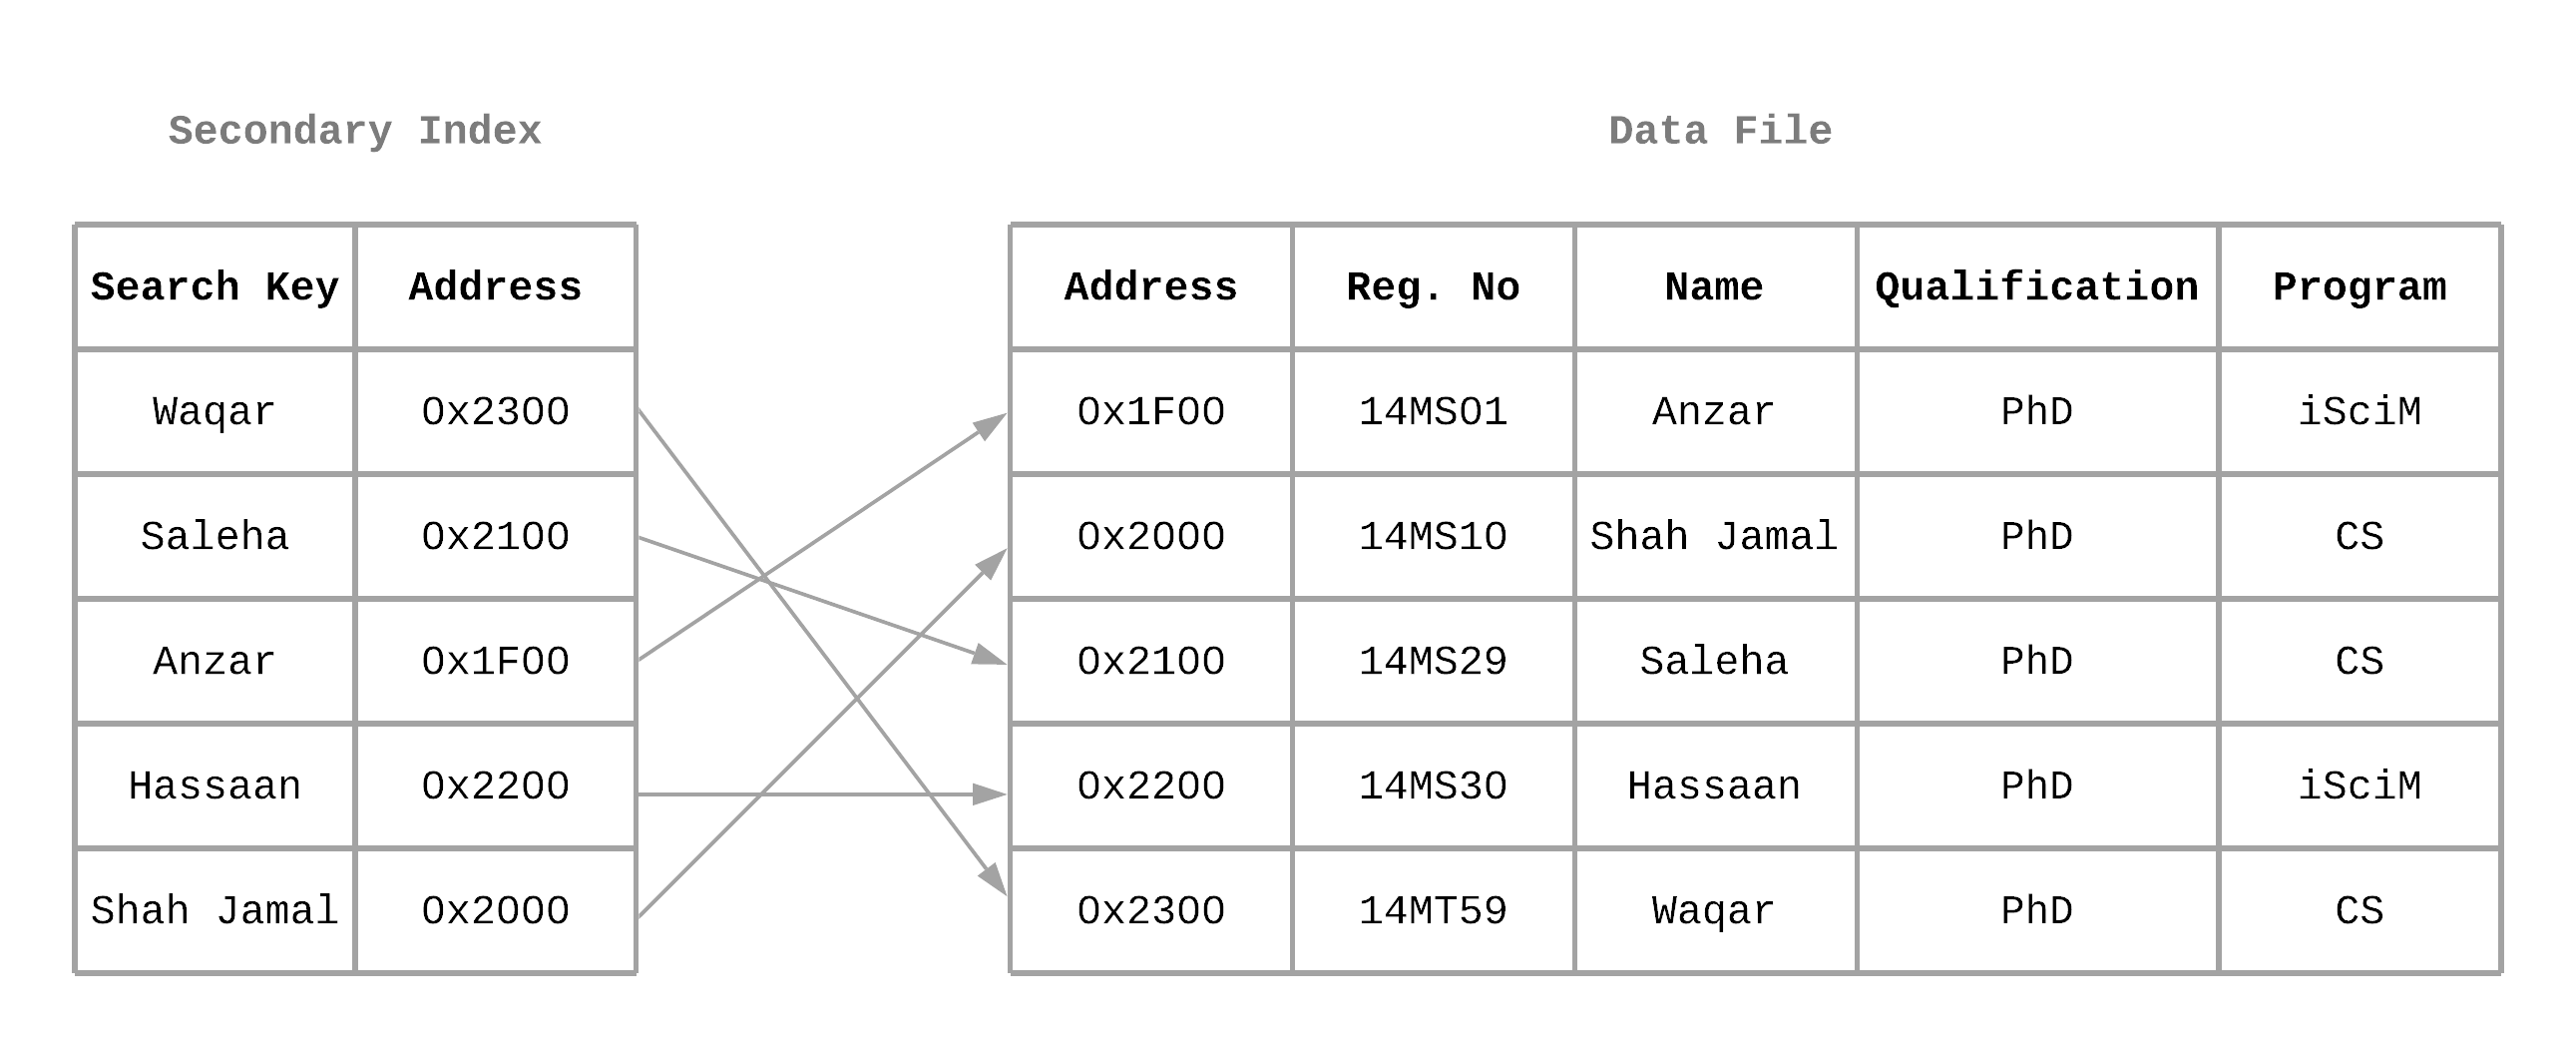
\includegraphics[width=.8\linewidth]{index}
  \caption{An index over the Name attribute of a table. The index stores values of the Name attribute as keys with the associated value being the address of the corresponding record in the table.}
  \label{fig:index}
\end{figure}

You have learned about database indexes in CS 355 Database Systems. Indexes in databases are similar to indexes in books. In a book, an index allows you to find information quickly without reading the entire book. In a database, an index allows the database program to find data in a table without scanning the entire table. An index in a book is a sorted list of words with the page numbers that contain each word. An index in a database is a sorted list of key values with the storage locations of rows in the table that contain the key value. Each key in the index is associated with a particular pointer to a record in the data file. Figure \ref{fig:index} shows an index on the \textit{Name} attribute of an \textit{Instructor} table stored in a data file. Note that key values in the figure are not sorted.

The most popular data structure used for indexing in relational databases is Btree (or its variant, such as B+tree). Btrees rose to popularity because they do fewer disk I/O operations to run a lookup compared to other balanced trees. SingleStore is the first commercial relational database in production today to use a skiplist, not a Btree, as its primary index data structure for in-memory data \cite{singlestore}.

You are given a data file, \texttt{data/books.csv}, that contains records of books. Each record contains the following attributes:
\begin{itemize}
  \item Book Code
  \item Title
  \item Category
  \item Price
  \item Number of Pages
\end{itemize}
For some of the attributes, all the values are unique. Such attributes can be used to index the table. Others have repeating values and are thus unsuitable to be used for indexing.

\section{Implementation Details and Tasks}

You are required to provide the missing implementations for the methods in the files, \texttt{skiplist.py} and \texttt{db.py}, in the accompanying \texttt{src/} sub-folder. \texttt{skiplist.py} contains classes to implement a skiplist. \texttt{db.py} contains a \pyth{Table} class to store records which can be indexed using a skiplist. Every individual field in the \pyth{Table} is stored as strings. Further details are provided in the doc strings in the files. The methods to be implemented are identified with a \pyth{pass} in their body.

\subsection{Requirement}

You will need to install the \pyth{typing} module to support certain type hints used in the code.

\subsection{Tips}

Below are some tips to avoid the errors that have previously caused tests to fail. Following these may save you many frustrating hours of debugging!
\begin{itemize}
  \item Store each field that is read from file as a \pyth{str}.
  \item Store a record as a list of field values.
  \item Store a table as a collection of records.
  \item Make sure that the \pyth{Table} can be re-indexed during run-time.
  \item Take care that the keys for the index are the values of the specified attribute. And that the value associated with each key is not the corresponding record, but a means to locate the record in the table.
  \item For the \pyth{select_range} query, think of an approach better than submitting multiple \pyth{select} queries.
\end{itemize}

\subsection{Testing}

Once you have successfully implemented the methods, you can test your code by reading from the accompanying data file, \texttt{data/books.csv}, and performing queries on it. For grading purposes, your submission will be tested automatically by GitHub using the accompanying \pyth{pytest} file, \texttt{test\_index.py}.

\newpage


\newpage
\newpage
\begin{thebibliography}{9}

  \bibitem{singlestore}
  The Story Behind SingleStore’s Skiplist Indexes, \url{https://www.singlestore.com/blog/what-is-skiplist-why-skiplist-index-for-memsql/}, last accessed on 16 Feb 2022.
  \end{thebibliography}
\end{document}
%%% Local Variables:
%%% mode: latex
%%% TeX-master: t
%%% End:
